%!TEX program = pdflatex
%----------------------------------------------------------------------------------------------------------------------
% Author: Jonas Nygaard Eriksen
% Encoding: UTF8
% LaTeX File for "Expected Business Conditions and Bond Risk Premia" 
% Last modified: December, 2015
%----------------------------------------------------------------------------------------------------------------------
% PREAMBLE
%----------------------------------------------------------------------------------------------------------------------

% Require the nag package to warn about obsolete stuff
\RequirePackage[l2tabu,orthodox]{nag}

% Formatting JFQA requirements
% \documentclass[12pt,letterpaper,leqno,doublespacing]{article}
% \usepackage[left=1in,right=1in,top=1in,bottom=1in]{geometry}
% \usepackage{setspace}  
% \usepackage{footmisc}
% \renewcommand{\footnotelayout}{\doublespacing}
% \setlength{\footnotesep}{0.5cm}
% \makeatletter
%     \renewcommand\@seccntformat[1]{\csname the#1\endcsname.\quad}
% \makeatother
% \renewcommand{\thesection}{\Roman{section}}
% \renewcommand{\thesubsection}{\Alph{subsection}}
% \renewcommand{\thesubsubsection}{\Alph{subsection}.\arabic{subsubsection}}

% Setting document class, font, font size, and bibliography op tions
\documentclass[12pt,a4paper,onecolumn,oneside,notitlepage]{article}
\usepackage[left=2.5cm,right=2.5cm,top=2.5cm,bottom=2.5cm]{geometry}
\usepackage[onehalfspacing]{setspace}

% Setting bibliography and typography options
\usepackage[longnamesfirst]{natbib}
\usepackage[english]{babel}
\usepackage[utf8]{inputenc}
\usepackage{eucal}
\usepackage[T1]{fontenc}
\usepackage{hyphenat}
\usepackage{microtype}
\usepackage{verbatim}

% Loading math packages
\usepackage{amsmath}
\usepackage{amsfonts}
\usepackage{amssymb}
\usepackage{amsthm}

% Loading tables and figures packages
\usepackage{makeidx}
\usepackage{tabularx}
\usepackage{graphicx}
\usepackage{epstopdf}
\usepackage{booktabs}
\usepackage{lscape}
\usepackage{longtable}
\usepackage{seqsplit}
\usepackage{rotating}
\usepackage{multicol}

% Loading auxiliary packages
\usepackage{soul}
\usepackage{blindtext}
\usepackage{appendix}

% Setting caption options
\usepackage{caption}
\usepackage{subcaption}
\captionsetup{
    labelfont = bf,
    labelsep = colon
}

% Setting coloring of links and references
\usepackage{hyperref}
\usepackage{xcolor}
\definecolor{au_blue}{RGB}{5,61,115}
\definecolor{navy_blue}{RGB}{0,0,128}
\definecolor{dark_red}{RGB}{153,0,0}
\definecolor{stylish_brown}{RGB}{188,90,100}
\definecolor{dark_orange}{RGB}{233,129,45}
\hypersetup{
    colorlinks=true,
    breaklinks=true,
    bookmarksnumbered=true,
    bookmarksopen=true,
    bookmarksdepth=2,
    citecolor=dark_red,
    linkcolor=dark_red,
    urlcolor=navy_blue,
    pdftitle={Expected Business Conditions and Bond Risk Premia},
    pdfauthor={Jonas Nygaard Eriksen}
}

% Setting up values for table creation
\renewcommand{\arraystretch}{0.95}
\newcolumntype{Y}{>{\centering\arraybackslash}X}
\newcolumntype{Z}{>{\raggedright\arraybackslash}X}

% SETTING BIBLIOGRAPHY PROPERTIES
\setlength{\bibsep}{0.1pt plus 0.3ex}

%----------------------------------------------------------------------------------------------------------------------
% FRONT MATTER
%----------------------------------------------------------------------------------------------------------------------

\begin{document}

% Defining title and footnotes
\pagenumbering{Alph}
\newcommand{\mytitle}{\textbf{\Large{Expected Business Conditions and Bond Risk Premia}} \\~\\ Tables and figures file}
\renewcommand{\refname}{References}
\long\def\symbolfootnote[#1]#2{\begingroup\def\thefootnote{\fnsymbol{footnote}}\footnote[#1]{#2}\endgroup}

% Setting up custom title page
\begin{titlepage}

    \thispagestyle{empty}
    \setlength{\parindent}{0cm}
    \begin{center}

        \small
        \renewcommand{\thefootnote}{\fnsymbol{footnote}}

        \vspace*{4cm} 
        \mytitle\symbolfootnote[1]{
            I am grateful to Stig Vinther Møller, Maik Schmeling, an anonymous referee, and seminar participants at Aarhus University and CREATES and the 2015 Nordic Econometric Meeting in Helsinki for helpful comments and suggestions. The author acknowledge support from CREATES - Center for Research in Econometric Analysis of Time Series (DNRF78), funded by the Danish National Research Foundation
        }

        \vspace*{2cm}
        \textbf{\normalsize{
            Jonas Nygaard Eriksen}\symbolfootnote[7]{CREATES, Department of Economics and Business Economics, Aarhus University, Fuglesangs All{\'e} 4, DK-8210 Aarhus V, Denmark. Tel.: +45 87165321. E-mail: \href{mailto:jeriksen@econ.au.dk}{jeriksen@econ.au.dk}.
            }
        }

        \vspace{1.2cm}
        {
            \normalsize  
            \vspace{1.5cm}
            This version: \today
        }
        \clearpage
        \thispagestyle{empty}
        \vspace*{2cm}
        \mytitle
        \vspace*{0.5cm}
        \begin{singlespace}
            \begin{abstract}
                \noindent This paper studies the predictability of bond risk premia by means of expectations to future business conditions using survey forecasts from the Survey of Professional Forecasters. We show that expected business conditions consistently affect excess bond returns and that the inclusion of expected business conditions in standard predictive regressions improve forecast performance relative to models using information derived from the current term structure or macroeconomic variables. The results are confirmed in a real-time out-of-sample exercise, where the predictive accuracy of the models is evaluated both statistically and from the perspective of a mean-variance investor that trades in the bond market.  \\\bigskip
                \noindent\textbf{Keywords:} Bond risk premia, expected business conditions, predictability, economic value, expectations hypothesis, time-varying risk premia\\\medskip
                \noindent\textbf{JEL Classification:} E43, E44, E47, G11, G12. \\\bigskip
                \noindent\textbf{This version:} \today
            \end{abstract}
        \end{singlespace}
    \end{center}        
\end{titlepage}

%----------------------------------------------------------------------------------------------------------------------
% INTRODUCTION
%----------------------------------------------------------------------------------------------------------------------

\clearpage
\setcounter{page}{1}
\pagenumbering{arabic}

%----------------------------------------------------------------------------------------------------------------------
% FIGURES
%----------------------------------------------------------------------------------------------------------------------

% SURVEY-EXPECTATIONS AND REALIZED MACRO-VARIABLES
\clearpage
\begin{figure}[htbp]
    \caption{
        \textbf{Estimated survey factors.} \newline
        This figure illustrates the time series dynamics of the survey factors estimated from the term structure of survey forecasts. The factors are plotted against National Bureau of Economic Research (NBER) recession periods marked in gray shading. The principal components are estimated using the full range of available observations covering the period 1968:Q4 to 2014:Q4. 
    }
    \centering
    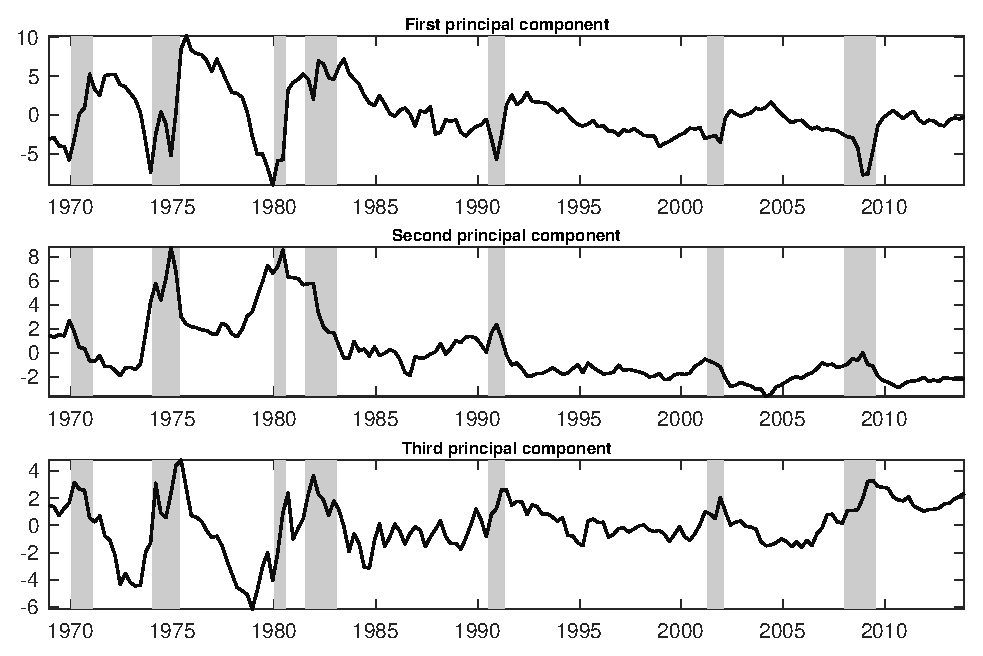
\includegraphics[scale=1]{Figures/e_principal_components.eps}
    \label{Fig:e_principal_components}
\end{figure}


% TIME SERIES DYNAMICS OF THE ME FACTORS
\clearpage
\begin{figure}[htbp]
    \caption{
        \textbf{Time series dynamics of the ME$_{t}$ factor.} \newline
        This figure illustrates the relation between expected business conditions $\left(\text{ME}_{t}\right)$ and the real economy as measured by the Chicago National Activity Index (CFNAI$_{t}$) and National Bureau of Economic Research (NBER) defined recession periods in gray shading over the sample period 1968:Q4-2014:Q4. ME$_{t}$ and CFNAI$_{t}$ are plotted in standardized units for convenience. 
    }
    \centering
    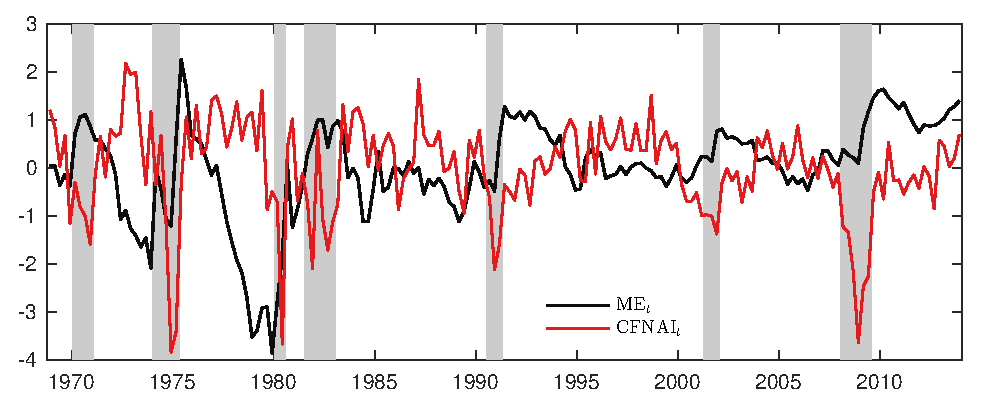
\includegraphics[scale=1]{Figures/e_me_cfnai.eps}
    \label{Fig:e_me_cfnai}
\end{figure}

% CUMULATIVE DIFFERENCES IN SQUARED FORECAST ERRORS
\clearpage
\begin{figure}[htbp]
    \caption{
        \textbf{Differences in cumulative squared prediction errors.} \newline
        This figure illustrates the relative forecasting performance by plotting the difference in cumulative squared prediction errors from (\ref{eq:e_dcsfe}) between the candidate forecasting model and the expectations hypothesis (EH) model  over the out-of-sample evaluation period, which covers the period from 1990:Q1 to 2014:Q4. National Bureau of Economic Research (NBER) recession periods are marked in gray shading.
    }
    \centering
    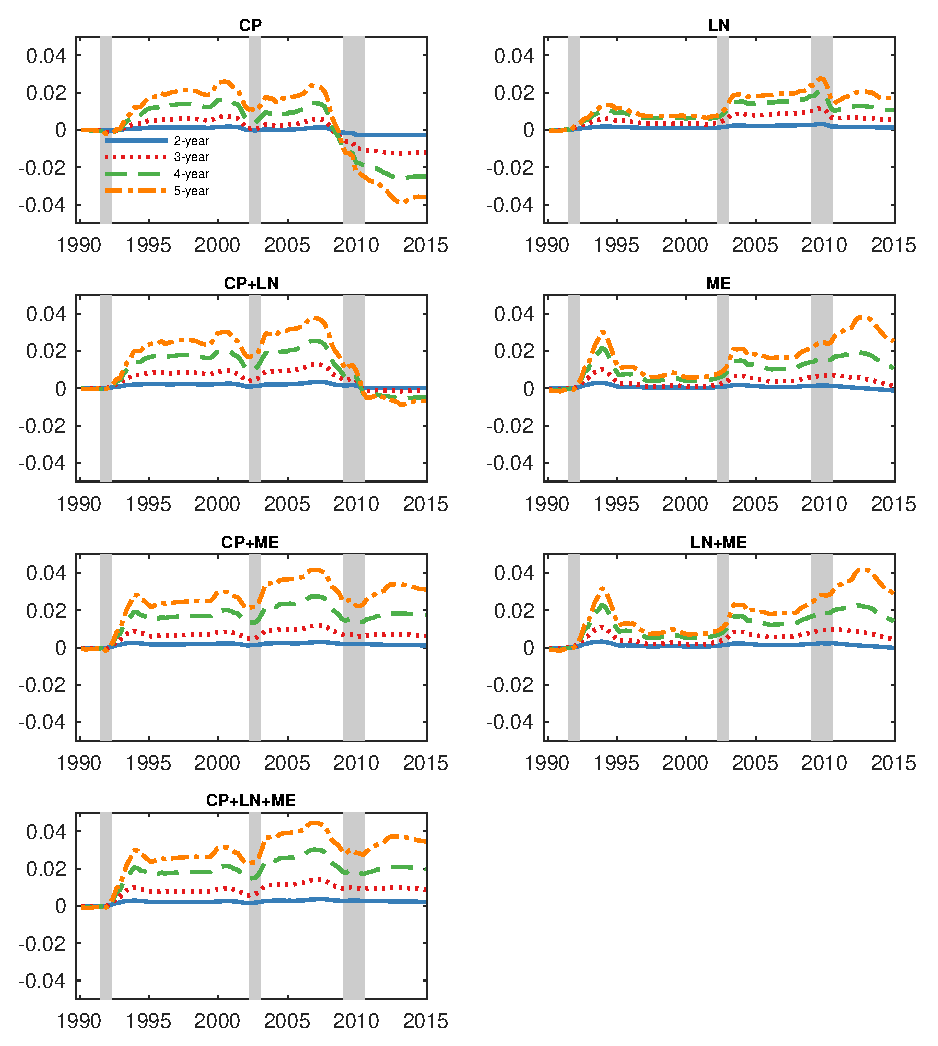
\includegraphics[scale=1]{Figures/e_dcsfe.eps}
    \label{Fig:e_dcsfe}
\end{figure}

% CUMULATIVE DIFFERENCES IN UTILITY GAINS
\clearpage
\begin{figure}[htbp]
    \caption{
        \textbf{Differences in cumulative realized utility.} \newline
        This figure illustrates the relative portfolio performance by plotting the difference in cumulative realized utility from (\ref{eq:e_average_utility}) between the candidate forecasting model and the expectations hypothesis (EH) model  over the out-of-sample evaluation period, which covers the period from 1990:Q1 to 2014:Q4. National Bureau of Economic Research (NBER) recession periods are marked in gray shading.
    }
    \centering
    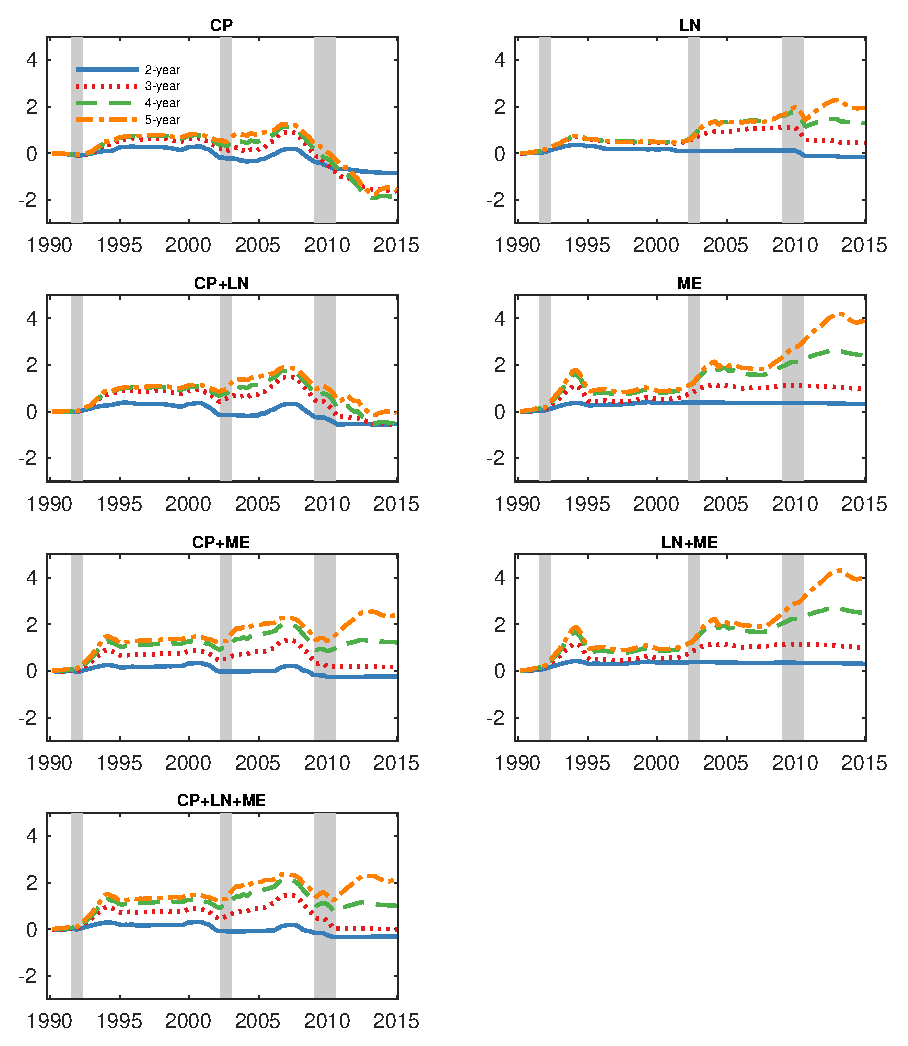
\includegraphics[scale=1]{Figures/e_dcutil.eps}
    \label{Fig:e_dcutil}
\end{figure}

%----------------------------------------------------------------------------------------------------------------------
% TABLES
%----------------------------------------------------------------------------------------------------------------------

% SUMMARY STATISTICS FOR SPF VARIABLES
\clearpage
\begin{table}[htbp]
    \footnotesize
    \caption{
        \textbf{Descriptive statistics: Survey variables.} \newline
        This table reports descriptive statistics for the median expected growth rates for the macroeconomic fundamentals collected from the Survey of Professional Forecasters (SPF). The variables include: 1) GDP $\left(\text{gdp}_{t}^{\mathbb{E}}\right)$, 2) the GDP price index $\left(\text{inf}_{t}^{\mathbb{E}}\right)$, 3) the unemployment rate $\left(\text{unemp}_{t}^{\mathbb{E}}\right)$, 4) corporate profits after tax $\left(\text{cprof}_{t}^{\mathbb{E}}\right)$, 5) industrial production $\left(\text{ip}_{t}^{\mathbb{E}}\right)$, and 6) housing starts $\left(\text{hous}_{t}^{\mathbb{E}}\right)$. We report means, standard deviations, skewness, and kurtosis for each fundamental and forecast horizon. The last three rows in each panel reports the loadings from the principal component estimation. The sample covers the period from 1968:Q4 to 2014:Q4.
    }
    \centering
    \begin{tabularx}{\textwidth}{ZYYYYYYYYYYY}
        \toprule
         & gdp$_{t}^{\mathbb{E}}$ & inf$_{t}^{\mathbb{E}}$ & cprof$_{t}^{\mathbb{E}}$ & unemp$_{t}^{\mathbb{E}}$ & ip$_{t}^{\mathbb{E}}$ & hous$_{t}^{\mathbb{E}}$ \\\midrule
 & \multicolumn{6}{c}{Panel A: One quarter ahead} \\\cmidrule{2-7}
Mean & 1.53 & 0.88 & 1.42 & 0.51 & 0.77 & 0.23 \\
Std & 0.57 & 0.50 & 2.11 & 2.74 & 0.79 & 5.67 \\
Skewness & 0.63 & 1.18 & -0.70 & 1.01 & -0.67 & -0.05 \\
Kurtosis & 3.18 & 3.55 & 5.46 & 3.31 & 5.79 & 4.42 \\
Load $\mathcal{P}_{1,t}^{\mathbb{E}}$ & 0.22 & 0.07 & 0.24 & -0.20 & 0.24 & 0.14 \\
Load $\mathcal{P}_{2,t}^{\mathbb{E}}$ & 0.18 & 0.36 & -0.16 & 0.20 & -0.15 & 0.06 \\
Load $\mathcal{P}_{3,t}^{\mathbb{E}}$ & -0.21 & -0.10 & -0.03 & 0.16 & -0.10 & 0.43 \\\cmidrule{2-7}
 & \multicolumn{6}{c}{Panel B: Two quarter ahead} \\\cmidrule{2-7}
Mean & 3.13 & 1.77 & 3.19 & 0.52 & 1.66 & 1.67 \\
Std & 1.11 & 0.97 & 3.50 & 4.78 & 1.32 & 10.12 \\
Skewness & 0.73 & 1.15 & -0.37 & 1.10 & -0.66 & 0.20 \\
Kurtosis & 2.95 & 3.49 & 4.95 & 3.74 & 5.87 & 3.79 \\
Load $\mathcal{P}_{1,t}^{\mathbb{E}}$ & 0.22 & 0.08 & 0.26 & -0.23 & 0.26 & 0.12 \\
Load $\mathcal{P}_{2,t}^{\mathbb{E}}$ & 0.21 & 0.36 & -0.12 & 0.19 & -0.12 & 0.11 \\
Load $\mathcal{P}_{3,t}^{\mathbb{E}}$ & -0.17 & -0.10 & 0.04 & 0.09 & -0.03 & 0.45 \\\cmidrule{2-7}
 & \multicolumn{6}{c}{Panel C: Three quarter ahead} \\\cmidrule{2-7}
Mean & 4.76 & 2.65 & 5.19 & -0.08 & 2.63 & 3.73 \\
Std & 1.62 & 1.42 & 4.45 & 5.81 & 1.64 & 14.32 \\
Skewness & 0.78 & 1.09 & 0.23 & 0.89 & -0.06 & 0.48 \\
Kurtosis & 2.83 & 3.36 & 4.02 & 3.29 & 4.38 & 3.69 \\
Load $\mathcal{P}_{1,t}^{\mathbb{E}}$ & 0.21 & 0.08 & 0.26 & -0.24 & 0.27 & 0.09 \\
Load $\mathcal{P}_{2,t}^{\mathbb{E}}$ & 0.23 & 0.36 & -0.07 & 0.17 & -0.08 & 0.16 \\
Load $\mathcal{P}_{3,t}^{\mathbb{E}}$ & -0.14 & -0.11 & 0.09 & 0.02 & 0.01 & 0.45 \\\cmidrule{2-7}
 & \multicolumn{6}{c}{Panel D: Four quarter ahead} \\\cmidrule{2-7}
Mean & 6.44 & 3.54 & 7.06 & -0.97 & 3.61 & 5.79 \\
Std & 2.15 & 1.86 & 5.09 & 6.55 & 1.91 & 17.78 \\
Skewness & 0.83 & 1.08 & 0.72 & 0.64 & 0.48 & 0.56 \\
Kurtosis & 2.78 & 3.34 & 3.56 & 2.79 & 3.88 & 3.60 \\
Load $\mathcal{P}_{1,t}^{\mathbb{E}}$ & 0.20 & 0.09 & 0.25 & -0.25 & 0.28 & 0.06 \\
Load $\mathcal{P}_{2,t}^{\mathbb{E}}$ & 0.26 & 0.35 & -0.01 & 0.14 & -0.04 & 0.19 \\
Load $\mathcal{P}_{3,t}^{\mathbb{E}}$ & -0.12 & -0.11 & 0.13 & -0.03 & 0.04 & 0.43 \\


        \bottomrule
        \label{Tab:e_sumstat_survey_variables}
    \end{tabularx}
\end{table}


% ESTIMATING THE MACRO-EXPECTATIONS FACTOR
\clearpage
\begin{table}[htbp]
    \footnotesize
    \caption{
        \textbf{Estimating the macroeconomic expectations factor.} \newline
        This table reports slope estimates from regressing one-year ahead bond risk premia upon the first three principal components ($\mathcal{P}_{1,t}^{\mathbb{E}}$,$\mathcal{P}_{2,t}^{\mathbb{E}}$,$\mathcal{P}_{3,t}^{\mathbb{E}}$) of the Survey of Professional Forecasters (SPF) forecasts and expected business conditions $\left(\text{ME}_{t}\right)$ in rows (a) and (b), respectively. Although not reported, all regressions contain an intercept. \cite{HansenHodrick1980} t-statistics implemented with four lags are presented in parentheses. Adj. R$^{2}\left(\%\right)$ denotes the full sample adjusted coefficient of determination in percentage. The sample period starts in 1968:Q4 and ends in 2014:Q4.
    }
    \centering
    \begin{tabularx}{\textwidth}{lYYYYYY}
        \toprule
         & $\mathcal{P}_{1,t}^{\mathbb{E}}$ & $\mathcal{P}_{2,t}^{\mathbb{E}}$ & $\mathcal{P}_{3,t}^{\mathbb{E}}$ & ME$_{t}$ & adj R$^{2}\left(\%\right)$ \\\midrule
 & \multicolumn{5}{c}{Panel A: Two-year bond} \\\cmidrule{2-6}
(a) & 0.08 & -0.10 & 0.38 &  & 18.87 \\
 & (2.03) & (-1.18) & (3.32) &  &  \\
(b) &  &  &  & 0.46 & 18.86 \\
 &  &  &  & (4.56) &  \\\cmidrule{2-6}
 & \multicolumn{5}{c}{Panel B: Three-year bond} \\\cmidrule{2-6}
(a) & 0.13 & -0.24 & 0.67 &  & 19.22 \\
 & (1.79) & (-1.58) & (3.49) &  &  \\
(b) &  &  &  & 0.86 & 19.85 \\
 &  &  &  & (4.71) &  \\\cmidrule{2-6}
 & \multicolumn{5}{c}{Panel C: Four-year bond} \\\cmidrule{2-6}
(a) & 0.20 & -0.43 & 0.83 &  & 18.99 \\
 & (2.03) & (-2.10) & (3.38) &  &  \\
(b) &  &  &  & 1.20 & 19.84 \\
 &  &  &  & (4.80) &  \\\cmidrule{2-6}
 & \multicolumn{5}{c}{Panel D: Five-year bond} \\\cmidrule{2-6}
(a) & 0.24 & -0.56 & 0.99 &  & 19.56 \\
 & (2.00) & (-2.42) & (3.57) &  &  \\
(b) &  &  &  & 1.47 & 20.29 \\
 &  &  &  & (4.90) &  \\


        \bottomrule
        \label{Tab:e_me_estimation}
    \end{tabularx}
\end{table}


% SUMMARY STATISTICS
\clearpage
\begin{table}[htbp]
    \footnotesize
    \caption{
        \textbf{Descriptive statistics: Bond risk premia and forecasting factors.} \newline
        This table reports descriptive statistics for excess bond returns $rx_{t+4}^{\left(n\right)}$, $n=2,\ldots,5$ and predictor variables used in the empirical analyses (Panel A) and their contemporaneous correlations (Panel B). CP$_{t}$ is the forward rate-based factor from \cite{CochranePiazzesi2005}, LN$_{t}$ is the macro-based factor from \cite{LudvigsonNg2009}, and ME$_{t}$ represents our proxy for expected business conditions described in Section \ref{Sec:e_measuring_ebc}. For each variable, we report means, standard deviations, skewness, and kurtosis as well as first- and second-order autocorrelations. In addition, we report Sharpe ratios (SR) for each of the Treasury bonds. The sample covers the period from 1968:Q4 to 2014:Q4.
    }
    \centering
    \begin{tabularx}{\linewidth}{ZYYYYYYYY}
        \toprule
         & $rx^{\left(2\right)}_{t+4}$ & $rx^{\left(3\right)}_{t+4}$ & $rx^{\left(4\right)}_{t+4}$ & $rx^{\left(5\right)}_{t+4}$ & CP$_{t}$ & LN$_{t}$ & ME$_{t}$ \\\midrule
 & \multicolumn{7}{c}{Panel A: Descriptive statistics} \\\cmidrule{2-8}
Mean & 0.60 & 1.06 & 1.48 & 1.63 & 1.19 & 1.19 & 1.19 \\
Std & 1.79 & 3.27 & 4.54 & 5.52 & 1.54 & 1.56 & 1.70 \\
Skewness & -0.24 & -0.29 & -0.28 & -0.20 & -0.10 & -0.72 & -1.22 \\
Kurtosis & 3.73 & 3.72 & 3.76 & 3.44 & 3.80 & 5.79 & 5.48 \\
AC(1) & 0.75 & 0.74 & 0.75 & 0.74 & 0.68 & 0.57 & 0.89 \\
AC(4) & 0.20 & 0.15 & 0.14 & 0.10 & 0.42 & 0.13 & 0.62\\
SR & 0.34 & 0.33 & 0.33 & 0.30 & - & - & - \\\cmidrule{2-8}
 & \multicolumn{7}{c}{Panel B: Correlation matrix} \\\cmidrule{2-8}
$rx^{\left(2\right)}_{t+4}$ & 1.00 &  &  &  &  &  &  \\
$rx^{\left(3\right)}_{t+4}$ & 0.98 & 1.00 &  &  &  &  &  \\
$rx^{\left(4\right)}_{t+4}$ & 0.96 & 0.99 & 1.00 &  &  &  &  \\
$rx^{\left(5\right)}_{t+4}$ & 0.93 & 0.97 & 0.99 & 1.00 &  &  &  \\
CP$_{t}$ & 0.37 & 0.40 & 0.43 & 0.40 & 1.00 &  &  \\
LN$_{t}$ & 0.41 & 0.43 & 0.42 & 0.40 & 0.11 & 1.00 &  \\
ME$_{t}$ & 0.44 & 0.45 & 0.45 & 0.46 & 0.42 & 0.33 & 1.00 \\


        \bottomrule
        \label{Table:e_sumstat_brp_factor}
    \end{tabularx}
\end{table}

% JOSLIN-PRIEBSCH-SINGLETON MACRO-SPANNING CONDITION
\clearpage
\begin{table}[htbp]
    \footnotesize
    \caption{
        \textbf{Macro-spanning condition for expected business conditions.} \newline
        This table reports slope estimates from the \cite{JoslinPriebschSingleton2014} macro-spanning condition in (\ref{eq:e_macro_spanning_condition}). Although not reported, all regressions contain an intercept. $\mathcal{P}_{1,t}^{\mathbb{E}}$, $\mathcal{P}_{2,t}^{\mathbb{E}}$, and $\mathcal{P}_{3,t}^{\mathbb{E}}$ denote the first three principal components estimated from survey forecasts and level$_{t}$, slope$_{t}$, curv$_{t}$, $\mathcal{Y}_{4,t}$, and $\mathcal{Y}_{5,t}$ are the principal components of the yield covariance matrix. \cite{NeweyWest1987} t-statistics implemented with six lags are presented in parentheses. Adj. R$^{2}\left(\%\right)$ denotes the full sample adjusted coefficient of determination in percentage. The sample period starts in 1968:Q4 and ends in 2014:Q4.
    }
    \centering
    \begin{tabularx}{\textwidth}{ZYYYYYYc}
        \toprule
         & Variable & level$_{t}$ & slope$_{t}$ & curv$_{t}$ & $\mathcal{Y}_{4,t}$ & $\mathcal{Y}_{5,t}$ & adj R$^{2}\left(\%\right)$ \\\midrule
(a) & $\mathcal{P}_{1,t}^{\mathbb{E}}$ & 0.12 & 2.51 & -0.55 &  &  & 28.15 \\
 &  & (1.82) & (4.35) & (-0.16) &  &  &  \\
(b) &  & 0.12 & 2.51 & -0.55 & -0.51 & 4.28 & 27.87 \\
 &  & (1.88) & (4.46) & (-0.16) & (-0.10) & (0.77) &  \\\cmidrule{2-8}
(a) & $\mathcal{P}_{2,t}^{\mathbb{E}}$ & 0.25 & -1.16 & 4.97 &  &  & 60.67 \\
 &  & (8.36) & (-3.46) & (2.75) &  &  &  \\
(b) &  & 0.26 & -1.16 & 4.97 & 0.27 & 7.42 & 62.97 \\
 &  & (8.66) & (-3.55) & (3.07) & (0.09) & (3.54) &  \\\cmidrule{2-8}
(a) & $\mathcal{P}_{3,t}^{\mathbb{E}}$ & -0.07 & 0.54 & 2.22 &  &  & 10.57 \\
 &  & (-1.42) & (1.53) & (1.72) &  &  &  \\
(b) &  & -0.07 & 0.54 & 2.24 & 6.17 & 5.31 & 17.75 \\
 &  & (-1.84) & (1.94) & (1.78) & (2.52) & (1.98) &  \\\cmidrule{2-8}
(a) & ME$_{t}$ & -0.12 & 1.19 & -0.14 &  &  & 42.17 \\
 &  & (-2.72) & (3.46) & (-0.20) &  &  &  \\
(b) &  & -0.12 & 1.19 & -0.13 & 4.27 & 2.05 & 45.23 \\
 &  & (-3.20) & (3.93) & (-0.14) & (1.68) & (1.13) &  \\


        \bottomrule
        \label{Tab:e_spanning_restriction}
    \end{tabularx}
\end{table}


% IN-SAMPLE RESULTS
\clearpage
\begin{table}[htbp]
    \scriptsize
    \caption{
        \textbf{In-sample results.} \newline
        This table reports slope estimates from regressing one-year ahead bond risk premia upon various combinations of predictors. CP$_{t}$ is the forward rate-based factor from \cite{CochranePiazzesi2005}, LN$_{t}$ is the macro-based factor from \cite{LudvigsonNg2009}, and ME$_{t}$ represents our proxy for expected business conditions described in Section \ref{Sec:e_measuring_ebc}. Although not reported, all regressions contain an intercept. \cite{HansenHodrick1980} t-statistics implemented with four lags are presented in parentheses. Adj. R$^{2}\left(\%\right)$ denotes the full sample adjusted coefficient of determination in percentage. The sample period starts in 1968:Q4 and ends in 2014:Q4.
    }
    \centering
    \begin{tabularx}{\textwidth}{lYYYYYYY}
        \toprule
         & CP$_{t}$ & LN$_{t}$ & ME$_{t}$ & adj R$^{2}\left(\%\right)$ \\\midrule
 & \multicolumn{4}{c}{Panel A: Two-year bond} \\\cmidrule{2-5}
(a) & 0.43 &  &  & 13.17 \\
 & (3.44) &  &  &  \\
(b) & 0.26 &  & 0.36 & 22.55 \\
 & (1.63) &  & (2.80) &  \\
(c) &  & 0.47 &  & 16.47 \\
 &  & (3.58) &  &  \\
(d) &  & 0.34 & 0.36 & 26.52 \\
 &  & (3.98) & (3.78) &  \\
(e) & 0.38 & 0.43 &  & 26.82 \\
 & (2.94) & (3.95) &  &  \\
(f) & 0.27 & 0.35 & 0.25 & 30.72 \\
 & (1.65) & (4.69) & (2.06) &  \\\cmidrule{2-5}
 & \multicolumn{4}{c}{Panel B: Three-year bond} \\\cmidrule{2-5}
(a) & 0.84 &  &  & 15.16 \\
 & (3.40) &  &  &  \\
(b) & 0.53 &  & 0.66 & 24.56 \\
 & (1.90) &  & (3.06) &  \\
(c) &  & 0.90 &  & 18.06 \\
 &  & (4.21) &  &  \\
(d) &  & 0.66 & 0.66 & 28.46 \\
 &  & (4.74) & (3.57) &  \\
(e) & 0.75 & 0.82 &  & 30.07 \\
 & (3.08) & (5.00) &  &  \\
(f) & 0.56 & 0.68 & 0.45 & 33.77 \\
 & (1.95) & (6.03) & (2.09) &  \\\cmidrule{2-5}
 & \multicolumn{4}{c}{Panel C: Four-year bond} \\\cmidrule{2-5}
(a) & 1.28 &  &  & 18.39 \\
 & (3.59) &  &  &  \\
(b) & 0.87 &  & 0.87 & 26.69 \\
 & (2.13) &  & (2.95) &  \\
(c) &  & 1.22 &  & 17.10 \\
 &  & (4.25) &  &  \\
(d) &  & 0.89 & 0.93 & 27.74 \\
 &  & (4.53) & (3.62) &  \\
(e) & 1.16 & 1.10 &  & 32.12 \\
 & (3.24) & (5.15) &  &  \\
(f) & 0.91 & 0.92 & 0.58 & 35.28 \\
 & (2.15) & (5.79) & (1.92) &  \\\cmidrule{2-5}
 & \multicolumn{4}{c}{Panel D: Five-year bond} \\\cmidrule{2-5}
(a) & 1.45 &  &  & 15.93 \\
 & (3.16) &  &  &  \\
(b) & 0.93 &  & 1.12 & 25.38 \\
 & (1.78) &  & (3.01) &  \\
(c) &  & 1.40 &  & 15.25 \\
 &  & (4.48) &  &  \\
(d) &  & 0.98 & 1.18 & 26.78 \\
 &  & (4.56) & (3.67) &  \\
(e) & 1.31 & 1.26 &  & 28.21 \\
 & (2.85) & (5.18) &  &  \\
(f) & 0.97 & 1.01 & 0.80 & 32.41 \\
 & (1.79) & (5.33) & (2.04) &  \\


        \bottomrule
        \label{Tab:e_insample_results}
    \end{tabularx}
\end{table}

% OUT-OF-SAMPLE RESULTS
\clearpage
\begin{table}[htbp]
    \footnotesize
    \caption{
        \textbf{Out-sample-results.} \newline
        This table reports the out-of-sample results from forecasting one-year ahead bond risk premia using various combinations of predictors. CP$_{t}$ is the forward rate-based factor from \cite{CochranePiazzesi2005}, LN$_{t}$ is the macro-based factor from \cite{LudvigsonNg2009}, and ME$_{t}$ represents our proxy for expected business conditions described in Section \ref{Sec:e_measuring_ebc}. Panel A reports the \cite{CampbellThompson2008} R$^{2}_{oos}$ statistic from (\ref{eq:e_r2oos}) relative to the expectations hypothesis (EH) benchmark accompanied by p-values from \cite{ClarkWest2007} tests of equal predictive ability in square brackets. Panel B reports annualized percentage utility gain, $\Delta\left(\%\right)$, relative to the EH model accompanied by p-valued from \cite{DieboldMariano1995} tests of equal utilities in square brackets. Finally, Panel C reports annualized \cite{GoetzmannIngersollSpiegelWelch} manipulation-proof performance measures, $\Theta\left(\%\right)$. The out-of-sample evaluation period starts in 1990:Q1 and ends in 2014:Q4.
    }
    \centering
    \begin{tabularx}{\textwidth}{lYYYYYYY}
        \toprule
        n & CP & LN & CP+LN & ME & CP+ME & LN+ME & CP+LN+ME \\\midrule
 & \multicolumn{7}{c}{Panel A: R$^{2}_{\text{oos}}$} \\\cmidrule{2-8}
2 & -16.26 & 7.57 & 0.80 & -7.17 & 6.53 & -1.13 & 12.31 \\
 & [0.17] & [0.01] & [0.02] & [0.07] & [0.04] & [0.05] & [0.03] \\
3 & -20.10 & 9.08 & -2.05 & 2.08 & 10.15 & 6.99 & 14.54 \\
 & [0.24] & [0.01] & [0.04] & [0.03] & [0.03] & [0.02] & [0.02] \\
4 & -20.27 & 8.77 & -3.98 & 8.77 & 14.06 & 11.51 & 16.09 \\
 & [0.20] & [0.01] & [0.05] & [0.02] & [0.02] & [0.02] & [0.02] \\
5 & -18.62 & 8.82 & -3.54 & 13.08 & 16.12 & 15.05 & 17.86 \\
 & [0.28] & [0.01] & [0.07] & [0.01] & [0.02] & [0.01] & [0.02] \\\cmidrule{2-8}
 & \multicolumn{7}{c}{Panel B: $\Delta\left(\%\right)$} \\\cmidrule{2-8}
2 & -0.84 & -0.15 & -0.54 & 0.32 & -0.23 & 0.31 & -0.31 \\
 & [0.97] & [0.75] & [0.88] & [0.01] & [0.75] & [0.02] & [0.82] \\
3 & -1.64 & 0.43 & -0.57 & 0.96 & 0.16 & 0.99 & -0.00 \\
 & [0.98] & [0.17] & [0.77] & [0.04] & [0.40] & [0.04] & [0.50] \\
4 & -1.95 & 1.28 & -0.56 & 2.39 & 1.21 & 2.46 & 0.99 \\
 & [0.99] & [0.02] & [0.74] & [0.00] & [0.06] & [0.00] & [0.11] \\
5 & -1.57 & 1.93 & -0.09 & 3.85 & 2.38 & 3.95 & 2.10 \\
 & [0.97] & [0.00] & [0.53] & [0.00] & [0.00] & [0.00] & [0.01] \\\cmidrule{2-8}
 & \multicolumn{7}{c}{Panel C: $\Theta\left(\%\right)$} \\\cmidrule{2-8}
2 & -0.90 & -0.03 & -0.61 & 0.47 & -0.27 & 0.46 & -0.34 \\
3 & -1.40 & 0.76 & -0.37 & 1.34 & 0.27 & 1.39 & 0.18 \\
4 & -1.42 & 1.56 & -0.14 & 2.86 & 1.41 & 2.97 & 1.30 \\
5 & -1.06 & 2.06 & 0.40 & 4.01 & 2.51 & 4.19 & 2.39 \\


        \bottomrule
        \label{Tab:e_out_of_sample_results}
    \end{tabularx}
\end{table}

% MODEL COMPARISONS
\clearpage
\begin{table}[htbp]
    \footnotesize
    \caption{
        \textbf{Model Comparisons.} \newline
        This table reports the out-of-sample results from forecasting one-year ahead bond risk premia using nested models with and without expected business conditions $\left(\text{ME}_{t}\right)$. R$^{2}_{\text{oos}}$ is the out-of-sample R$^{2}$ suggested in \cite{CampbellThompson2008}. For each R$^{2}_{\text{oos}}$, we report p-values from the \cite{ClarkWest2007} test of equal predictive ability in square brackets. $\Delta\left(\%\right)$ denotes the annualized percentage utility gain between the model including expected business conditions and the nested benchmark omitting expected business conditions. $\Theta\left(\%\right)$ is the annualized manipulation-proof measure from \cite{GoetzmannIngersollSpiegelWelch}. For each $\Delta\left(\%\right)$, we report p-values from the \cite{DieboldMariano1995} test in square brackets. The out-of-sample evaluation period starts in 1990:Q1 and ends in 2014:Q4.
    }
    \centering
    \begin{tabularx}{\textwidth}{lYYYYYYYYYY}
        \toprule
         & R$^{2}_{\text{oos}}$ & p-val & $\Delta$(\%) & p-val & $\Theta$(\%) \\\midrule
 & \multicolumn{5}{c}{Panel A: Two-year bond} \\\cmidrule{2-6}
CP+ME vs. CP & 19.60 & [0.00] & 0.61 & [0.03] & 0.63  \\
LN+ME vs. LN & -9.41 & [0.16] & 0.46 & [0.01] & 0.49 \\
CP+LN+ME vs. CP+LN & 11.60 & [0.02] & 0.23 & [0.19] & 0.27 \\\cmidrule{2-6}
 & \multicolumn{5}{c}{Panel B: Three-year bond} \\\cmidrule{2-6}
CP+ME vs. CP & 25.19 & [0.00] & 1.80 & [0.00] & 1.67 \\
LN+ME vs. LN & -2.30 & [0.11] & 0.55 & [0.13] & 0.62 \\
CP+LN+ME vs. CP+LN & 16.25 & [0.01] & 0.57 & [0.07] & 0.56 \\\cmidrule{2-6}
 & \multicolumn{5}{c}{Panel C: Four-year bond} \\\cmidrule{2-6}
CP+ME vs. CP & 28.54 & [0.00] & 3.16 & [0.00] & 2.83 \\
LN+ME vs. LN & 3.00 & [0.07] & 1.18 & [0.05] & 1.41 \\
CP+LN+ME vs. CP+LN & 19.30 & [0.00] & 1.56 & [0.00] & 1.44 \\\cmidrule{2-6}
 & \multicolumn{5}{c}{Panel D: Five-year bond} \\\cmidrule{2-6}
CP+ME vs. CP & 29.28 & [0.00] & 3.95 & [0.00] & 3.58 \\
LN+ME vs. LN & 6.83 & [0.05] & 2.02 & [0.01] & 2.13 \\
CP+LN+ME vs. CP+LN & 20.67 & [0.00] & 2.19 & [0.00] & 2.00 \\


        \bottomrule
        \label{Tab:e_out_of_sample_model_comparison}
    \end{tabularx}
\end{table}

 
% OUT-OF-SAMPLE FORECAST COMBINATION RESULTS
\clearpage
\begin{table}[htbp]
    \footnotesize
    \caption{
        \textbf{Forecast combination.} \newline
        This table reports the out-of-sample results from forecasting one-year ahead bond risk premia using combinations of forecasts. Panel A presents the results from combining forecasts from the three CP$_{t}$ and LN$_{t}$ models and Panel B presents the results from combining forecasts for all seven model. R$^{2}_{\text{oos}}$ is the out-of-sample R$^{2}$ suggested in \cite{CampbellThompson2008}. For each R$^{2}_{\text{oos}}$, we report p-values from the \cite{ClarkWest2007} test of equal predictive ability in square brackets. $\Delta\left(\%\right)$ denotes the annualized percentage utility gain between the model including expected business conditions and the nested benchmark omitting expected business conditions. $\Theta\left(\%\right)$ is the annualized manipulation-proof measure from \cite{GoetzmannIngersollSpiegelWelch}. For each $\Delta\left(\%\right)$, we report p-values from the \cite{DieboldMariano1995} test in square brackets. The out-of-sample evaluation period starts in 1990:Q1 and ends in 2014:Q4.
    }
    \centering
    \begin{tabularx}{\textwidth}{lYYYYYYYYYYYYYY}
        \toprule
        n & R$^{2}_{\text{oos}}$ & p-val & $\Delta$(\%) & p-val & $\Theta$(\%) \\\midrule
 & \multicolumn{5}{c}{Panel A: Forecast combination using CP$_{t}$ and LN$_{t}$ models} \\\cmidrule{2-6}
2 & 8.00 & [0.02] & -0.41 & [0.85] & -0.46 \\
3 & 5.98 & [0.04] & -0.50 & [0.76] & -0.39 \\
4 & 5.05 & [0.04] & -0.50 & [0.74] & -0.22 \\
5 & 3.85 & [0.06] & -0.07 & [0.53] & 0.21 \\\cmidrule{2-6}
 & \multicolumn{5}{c}{Panel B: Forecast combination using all models} \\\cmidrule{2-6}
2 & 15.81 & [0.02] & 0.13 & [0.28] & 0.16 \\
3 & 17.71 & [0.02] & 0.42 & [0.23] & 0.61 \\
4 & 19.60 & [0.01] & 1.22 & [0.04] & 1.39 \\
5 & 19.41 & [0.01] & 2.11 & [0.00] & 2.17 \\


        \bottomrule
        \label{Tab:e_forecast_combination}
    \end{tabularx}
\end{table}


% % CORRELATION MEASURES OF FORECASTING PERFORMANCE
\clearpage
\begin{table}[htbp]
    \footnotesize
    \caption{
        \textbf{Forecast performance, expected returns, and economic variables.} \newline
        This table reports contemporaneous correlations between relative forecast and portfolio performance and the real economy as measured by the Chicago Fed National Activity Index $\left(\text{CFNAI}_{t}\right)$ in Panels A and B. Relative forecast performance is defined as the difference in cumulative squared prediction error $\left(\text{DCSPE}_{t}\right)$ from (\ref{eq:e_dcsfe}) and portfolio performance is the cumulative difference in realized utilities $\left(\text{DCRU}_{t}\right)$ from (\ref{eq:e_average_utility}). Panels C and D report contemporaneous correlations between expected bond risk premia and the CFNAI$_{t}$ and macroeconomic uncertainty $\left(\mathbb{U}_{t}^{\text{Macro}}\right)$, respectively. Macro uncertainty is the uncertainty index constructed in \cite{JuradoLudvgisonNg2015}. The out-of-sample evaluation period starts in 1990:Q1 and ends in 2014:Q4.
    }
    \centering
    \begin{tabularx}{\textwidth}{lYYYYcYYYY}
        \toprule
         & 2-year & 3-year & 4-year & 5-year &  & 2-year & 3-year & 4-year & 5-year \\\midrule
 & \multicolumn{4}{c}{Panel A: $\rho\left(\text{DCSPE}_{t},\text{CFNAI}_{t}\right)$} &  & \multicolumn{4}{c}{Panel B: $\rho\left(\text{DCRU}_{t},\text{CFNAI}_{t}\right)$}  \\\cmidrule{2-5}\cmidrule{7-10}
CP & 0.53 & 0.49 & 0.47 & 0.44 &  & 0.48 & 0.37 & 0.30 & 0.26 \\
LN & -0.25 & -0.25 & -0.22 & -0.25 &  & 0.24 & -0.14 & -0.27 & -0.27 \\
CP+LN & 0.42 & 0.42 & 0.44 & 0.41 &  & 0.50 & 0.38 & 0.29 & 0.23 \\
ME & -0.31 & -0.42 & -0.32 & -0.26 &  & 0.02 & -0.28 & -0.27 & -0.24 \\
CP+ME & 0.16 & 0.24 & 0.29 & 0.23 &  & 0.54 & 0.45 & 0.31 & 0.14 \\
LN+ME & -0.41 & -0.42 & -0.32 & -0.27 &  & 0.04 & -0.28 & -0.27 & -0.25 \\
CP+LN+ME & 0.03 & 0.12 & 0.22 & 0.17 &  & 0.49 & 0.41 & 0.29 & 0.16 \\
FC1 & 0.25 & 0.30 & 0.33 & 0.32 &  & 0.50 & 0.38 & 0.31 & 0.24 \\
FC2 & -0.08 & -0.03 & 0.02 & 0.02 &  & 0.30 & 0.27 & 0.18 & 0.07 \\\cmidrule{2-5}\cmidrule{7-10}
 & \multicolumn{4}{c}{Panel C: $\rho\left(\mathbb{E}_{t}rx_{t+4}^{\left(n\right)},\text{CFNAI}_{t}\right)$} &  & \multicolumn{4}{c}{Panel D: $\rho\left(\mathbb{E}_{t}rx_{t+4}^{\left(n\right)},\mathbb{U}_{t}^{\text{Macro}}\right)$}  \\\cmidrule{2-5}\cmidrule{7-10}
CP & 0.03 & 0.02 & 0.03 & 0.02 &  & -0.24 & -0.23 & -0.24 & -0.23 \\
LN & -0.09 & -0.09 & -0.07 & -0.07 &  & -0.14 & -0.13 & -0.13 & -0.11 \\
CP+LN & -0.02 & -0.02 & 0.01 & 0.00 &  & -0.29 & -0.28 & -0.30 & -0.28 \\
ME & -0.43 & -0.43 & -0.42 & -0.42 &  & 0.18 & 0.20 & 0.20 & 0.20 \\
CP+ME & -0.29 & -0.27 & -0.23 & -0.26 &  & 0.02 & 0.02 & -0.03 & 0.01 \\
LN+ME & -0.37 & -0.37 & -0.34 & -0.36 &  & 0.06 & 0.07 & 0.06 & 0.10 \\
CP+LN+ME & -0.23 & -0.21 & -0.15 & -0.19 &  & -0.10 & -0.11 & -0.16 & -0.10 \\
FC1 & -0.03 & -0.03 & -0.00 & -0.01 &  & -0.28 & -0.27 & -0.28 & -0.26 \\
FC2 & -0.24 & -0.23 & -0.20 & -0.22 &  & -0.09 & -0.09 & -0.11 & -0.07 \\


        \bottomrule
        \label{Tab:e_links_to_the_real_economy}
    \end{tabularx}
\end{table}

% IN-SAMPLE RESULTS FOR GSW BOND DATA
\clearpage
\begin{table}[htbp]
    \caption{
        \textbf{In-sample results for quarterly bond risk premia.} \newline
        This table reports slope estimates from regressing one-quarter ahead bond risk premia upon various combinations of predictors. CP$_{t}^{\text{GSW}}$ is the forward rate-based factor from \cite{CochranePiazzesi2005}, LN$_{t}^{\text{GSW}}$ is the macro-based factor from \cite{LudvigsonNg2009}, and ME$_{t}^{\text{GSW}}$ represents our proxy for expected business conditions described in Section \ref{Sec:e_measuring_ebc}. Although not reported, all regressions contain an intercept. \cite{NeweyWest1987} t-statistics implemented with six lags are presented in parentheses. Adj. R$^{2}\left(\%\right)$ denotes the full sample adjusted coefficient of determination in percentage. The sample period starts in 1968:Q4 and ends in 2014:Q4.
    }
    \centering
    \scriptsize
    \begin{tabularx}{\textwidth}{lYYYYYYY}
        \toprule
         & CP$_{t}^{\text{GSW}}$ & LN$_{t}^{\text{GSW}}$ & ME$_{t}^{\text{GSW}}$ & adj R$^{2}\left(\%\right)$ \\\midrule
 & \multicolumn{4}{c}{Panel A: Two-year bond} \\\cmidrule{2-5}
(a) &  &  & 0.55 & 3.88 \\
 &  &  & (2.44) &  \\
(b) & 0.65 &  & 0.57 & 8.90 \\
 & (3.20) &  & (2.21) &  \\
(c) &  & 0.64 & 0.53 & 9.29 \\
 &  & (5.04) & (2.62) &  \\
(d) & 0.57 & 0.60 &  & 10.43 \\
 & (2.67) & (4.12) &  &  \\
(e) & 0.59 & 0.58 & 0.54 & 13.72 \\
 & (2.99) & (3.84) & (2.36) &  \\\cmidrule{2-5}
 & \multicolumn{4}{c}{Panel B: Three-year bond} \\\cmidrule{2-5}
(a) &  &  & 0.88 & 4.91 \\
 &  &  & (2.90) &  \\
(b) & 0.92 &  & 0.91 & 9.91 \\
 & (3.40) &  & (2.59) &  \\
(c) &  & 0.89 & 0.84 & 10.24 \\
 &  & (5.35) & (3.20) &  \\
(d) & 0.80 & 0.84 &  & 10.33 \\
 & (2.81) & (4.28) &  &  \\
(e) & 0.83 & 0.81 & 0.87 & 14.64 \\
 & (3.21) & (3.83) & (2.82) &  \\\cmidrule{2-5}
 & \multicolumn{4}{c}{Panel C: Four-year bond} \\\cmidrule{2-5}
(a) &  &  & 1.16 & 5.43 \\
 &  &  & (3.21) &  \\
(b) & 1.16 &  & 1.19 & 10.53 \\
 & (3.51) &  & (2.83) &  \\
(c) &  & 1.09 & 1.11 & 10.47 \\
 &  & (5.29) & (3.60) &  \\
(d) & 1.01 & 1.03 &  & 10.14 \\
 & (2.91) & (4.15) &  &  \\
(e) & 1.05 & 0.98 & 1.14 & 14.99 \\
 & (3.35) & (3.63) & (3.13) &  \\\cmidrule{2-5}
 & \multicolumn{4}{c}{Panel D: Five-year bond} \\\cmidrule{2-5}
(a) &  &  & 1.41 & 5.71 \\
 &  &  & (3.40) &  \\
(b) & 1.38 &  & 1.44 & 10.86 \\
 & (3.55) &  & (2.99) &  \\
(c) &  & 1.25 & 1.35 & 10.39 \\
 &  & (5.01) & (3.86) &  \\
(d) & 1.21 & 1.18 &  & 9.85 \\
 & (2.94) & (3.88) &  &  \\
(e) & 1.25 & 1.12 & 1.39 & 14.99 \\
 & (3.39) & (3.36) & (3.32) &  \\


        \bottomrule
        \label{Tab:e_insample_results_gsw_bonds}
    \end{tabularx}
\end{table}

%----------------------------------------------------------------------------------------------------------------------
% BIBLIOGRAPHY
%----------------------------------------------------------------------------------------------------------------------

\clearpage
\bibliographystyle{ecta}
\bibliography{e_refs}

%----------------------------------------------------------------------------------------------------------------------
% INTERNET APPENDIX
%----------------------------------------------------------------------------------------------------------------------

\clearpage
\phantomsection
\addcontentsline{toc}{section}{Internet Appendix}

\begin{appendices}

\begin{center}
    {
        \large Internet Appendix for \vspace{0.25cm}\\
        \mytitle \vspace{0.25cm}\\
        (not intended for publication) \vspace{0.25cm}\\
    }
\end{center}

% Setting up changes to layout for the appendix
\setcounter{page}{1}
\pagenumbering{roman}
\setcounter{section}{0}
\setcounter{subsection}{0}
\setcounter{equation}{0}
\renewcommand{\thesection}{IA.\Alph{section}}
\renewcommand{\thesubsection}{\thesection.\arabic{subsection}}
\renewcommand{\theequation}{IA.\arabic{equation}}
\renewcommand\thetable{IA.\arabic{table}} \setcounter{table}{0}
\renewcommand\thefigure{IA.\arabic{figure}} \setcounter{figure}{0}

%----------------------------------------------------------------------------------------------------------------------
% INFORMATIONAL CONTENT AT DIFFERENT FORECAST HORIZONS
%----------------------------------------------------------------------------------------------------------------------

\clearpage
\section{Predictive ability across forecast horizons}\label{sec:predictive_ability_across_forecast_horizons}
To better understand the predictive ability of survey forecasts for different forecast horizons, we construct horizon specific versions of the first three principal components $\left(\mathcal{P}_{1,t}^{\mathbb{E}},\mathcal{P}_{2,t}^{\mathbb{E}},\mathcal{P}_{3,t}^{\mathbb{E}}\right)$ and the macroeconomic expectations factor, ME$_{t}$, using data from the Survey of Professional Forecasters (SPF).
\begin{table}[htbp]
    \footnotesize
    \caption{
        \textbf{Predictive ability across forecast horizons.} \newline
        This table reports slope estimates from regressing one-year ahead bond risk premia upon horizon specific versions of the first three principal components ($\mathcal{P}_{1,t}^{\mathbb{E}}$,$\mathcal{P}_{2,t}^{\mathbb{E}}$,$\mathcal{P}_{3,t}^{\mathbb{E}}$) of the Survey of Professional Forecasters (SPF) forecasts and expected business conditions $\left(\text{ME}_{t}\right)$. Although not reported, all regressions contain an intercept. \cite{HansenHodrick1980} t-statistics implemented with four lags are presented in parentheses. Adj. R$^{2}\left(\%\right)$ denotes the full sample adjusted coefficient of determination in percentage. The sample period starts in 1968:Q4 and ends in 2014:Q4.
    }
    \centering
    \begin{tabularx}{\textwidth}{lYYYYYYYY}
        \toprule
         & $\mathcal{P}_{1,t}^{\mathbb{E}}$ & $\mathcal{P}_{2,t}^{\mathbb{E}}$ & $\mathcal{P}_{3,t}^{\mathbb{E}}$ & adj R$^{2}\left(\%\right)$ & ME$_{t}$ & adj R$^{2}\left(\%\right)$ \\\midrule
 & \multicolumn{6}{c}{Panel A: Two-year bond} \\\cmidrule{2-7}
One-quarter ahead & 0.13 & 0.21 & -0.77 & 20.08 & 0.47 & 19.97 \\
 & (1.44) & (1.42) & (-3.94) &  & (5.29) &  \\
Two-quarters ahead & 0.19 & 0.19 & -0.77 & 20.35 & 0.46 & 20.39 \\
 & (2.36) & (1.22) & (-3.62) &  & (5.35) &  \\
Three-quarters ahead & 0.16 & 0.22 & -0.75 & 18.58 & 0.46 & 18.63 \\
 & (2.27) & (1.31) & (-3.12) &  & (4.37) &  \\
Four-quarters ahead & 0.13 & 0.24 & -0.69 & 15.33 & 0.45 & 15.37 \\
 & (1.60) & (1.22) & (-2.58) &  & (3.23) &  \\\cmidrule{2-7}
 & \multicolumn{6}{c}{Panel B: Three-year bond} \\\cmidrule{2-7}
One-quarter ahead & 0.22 & 0.51 & -1.31 & 19.43 & 0.86 & 20.05 \\
 & (1.46) & (1.82) & (-3.88) &  & (5.26) &  \\
Two-quarters ahead & 0.32 & 0.46 & -1.37 & 20.70 & 0.86 & 21.32 \\
 & (2.23) & (1.66) & (-3.83) &  & (5.51) &  \\
Three-quarters ahead & 0.27 & 0.51 & -1.35 & 19.31 & 0.86 & 19.95 \\
 & (1.91) & (1.75) & (-3.35) &  & (4.60) &  \\
Four-quarters ahead & 0.19 & 0.55 & -1.24 & 16.03 & 0.86 & 16.72 \\
 & (1.21) & (1.60) & (-2.73) &  & (3.40) &  \\\cmidrule{2-7}
 & \multicolumn{6}{c}{Panel C: Four-year bond} \\\cmidrule{2-7}
One-quarter ahead & 0.42 & 0.87 & -1.61 & 19.24 & 1.20 & 20.08 \\
 & (1.95) & (2.29) & (-3.82) &  & (5.39) &  \\
Two-quarters ahead & 0.51 & 0.83 & -1.69 & 20.67 & 1.20 & 21.50 \\
 & (2.58) & (2.18) & (-3.79) &  & (5.68) &  \\
Three-quarters ahead & 0.38 & 0.91 & -1.66 & 19.03 & 1.20 & 19.88 \\
 & (2.05) & (2.25) & (-3.23) &  & (4.70) &  \\
Four-quarters ahead & 0.23 & 0.98 & -1.50 & 15.81 & 1.20 & 16.69 \\
 & (1.14) & (2.03) & (-2.52) &  & (3.44) &  \\\cmidrule{2-7}
 & \multicolumn{6}{c}{Panel D: Five-year bond} \\\cmidrule{2-7}
One-quarter ahead & 0.52 & 1.12 & -1.90 & 19.43 & 1.46 & 20.15 \\
 & (1.99) & (2.58) & (-4.02) &  & (5.35) &  \\
Two-quarters ahead & 0.63 & 1.08 & -2.02 & 21.12 & 1.47 & 21.84 \\
 & (2.57) & (2.52) & (-4.03) &  & (5.76) &  \\
Three-quarters ahead & 0.46 & 1.19 & -1.99 & 19.72 & 1.48 & 20.46 \\
 & (2.03) & (2.58) & (-3.42) &  & (4.84) &  \\
Four-quarters ahead & 0.27 & 1.27 & -1.82 & 16.69 & 1.49 & 17.46 \\
 & (1.13) & (2.30) & (-2.66) &  & (3.58) &  \\


        \bottomrule
        \label{Tab:e_horizon_specific_pcs}
    \end{tabularx}
\end{table}
We estimate the horizon specific principal components and ME$_{t}$ factors analogously to their full horizon counterparts in Section \ref{Sec:e_measuring_ebc}. The results, which are presented in Table \ref{Tab:e_horizon_specific_pcs}, show that the predictive ability of survey forecasts is not confined to a particular forecast horizon. In fact, albeit some heterogeneity is present in the loading sizes and significance, we see that the overall results are remarkably similar across forecast horizons. The pattern of loadings being an increasing function of bond maturity in absolute value emerges again and the same functions of horizon specific components forecast bond risk premia for all maturities. As such, we view our use of the full term structure of survey expectations as a way to average, in a sense, over the heterogeneities in the predictive abilities, thereby avoiding having to evaluate all possible combinations of components and forecast horizons in the SPF data. 

%----------------------------------------------------------------------------------------------------------------------
% THE TERM STRUCTURE OF EXPECTED BUSINESS CONDITIONS
%----------------------------------------------------------------------------------------------------------------------

\section{The term structure of survey forecasts}\label{sec:e_the_term_structure_of_expected_business_conditions}
The descriptive statistics in Section \ref{Sec:e_measuring_ebc} suggested that survey forecasts are extrapolative in the forecast horizon.  
\begin{figure}[tbp]
    \caption{
        \textbf{Term structure of expected business conditions.} \newline
        This figure plots one- through four-quarter ahead forecasts from the Survey of Professional Forecasters (SPF). The sample period starts in 1968:Q4 and ends in 2014:Q4.
    }
    \centering
    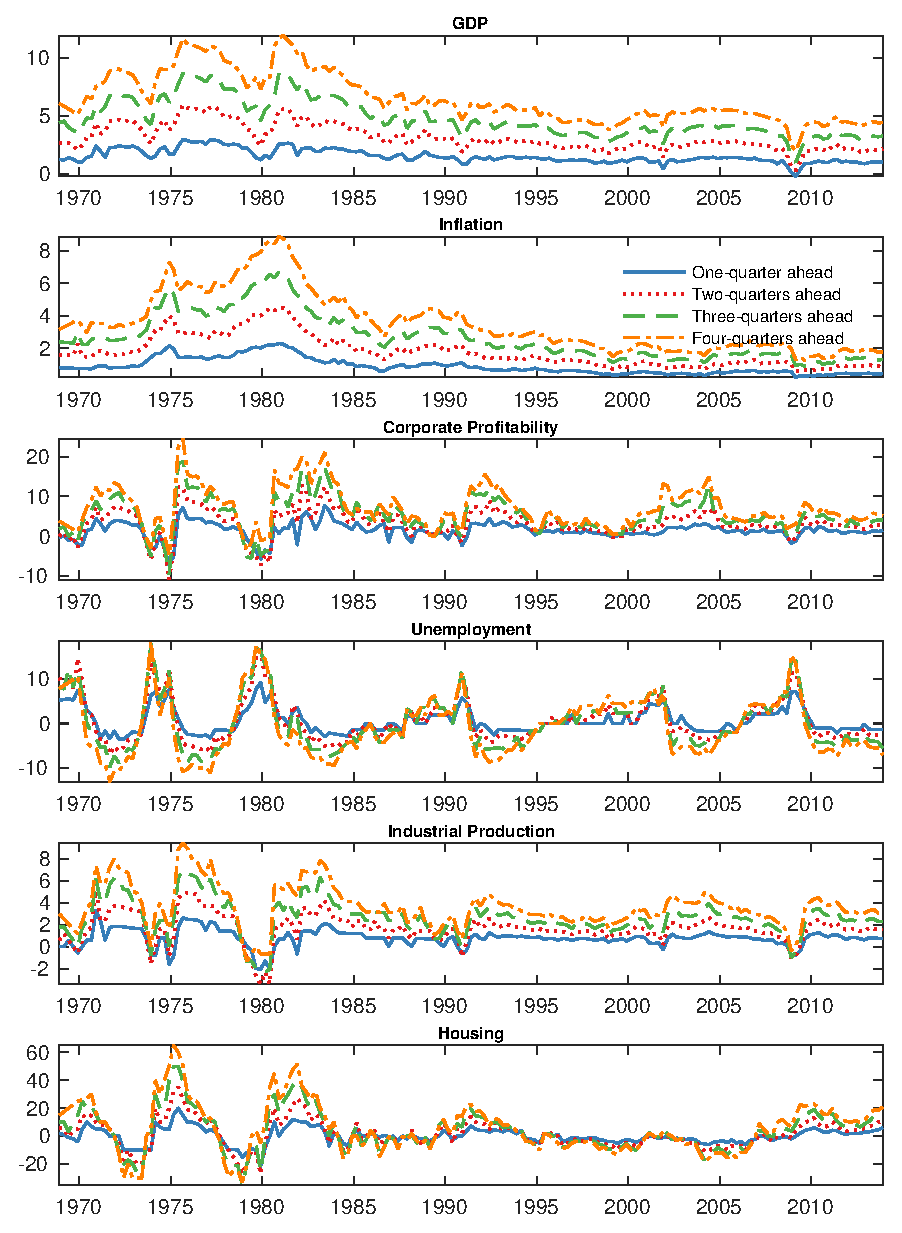
\includegraphics[scale=0.8]{Figures/e_survey_expectations.eps}
    \label{Fig:e_survey_expectations}
\end{figure}
As a verification, we plot in Figure \ref{Fig:e_survey_expectations} one- through four-quarter ahead forecasts from the SPF. As suggested by the descriptive statistics, we see that the majority of the forecasts are indeed displaying extrapolative behavior.

%----------------------------------------------------------------------------------------------------------------------
% VISUALIZING PRINCIPAL COMPONENT LOADINGS
%----------------------------------------------------------------------------------------------------------------------

\clearpage
\section{Visualizing principal component loadings}\label{sec:visualizing_principal_component_loaings}
While the loadings from the principal component analysis are tabulated in Table \ref{Tab:e_sumstat_survey_variables}, this section provides a visual interpretation by plotting the loadings in bar form in Figure \ref{Fig:e_pca_loadings}.
\begin{figure}[htbp]
    \caption{
        \textbf{Principal component loadings.} \newline
        This figure illustrates the loadings from the principal component analysis in Section \ref{Sec:e_measuring_ebc}. Loadings are grouped by macroeconomic fundamentals and ordered from shortest to longest forecast horizon. 
    }
    \centering
    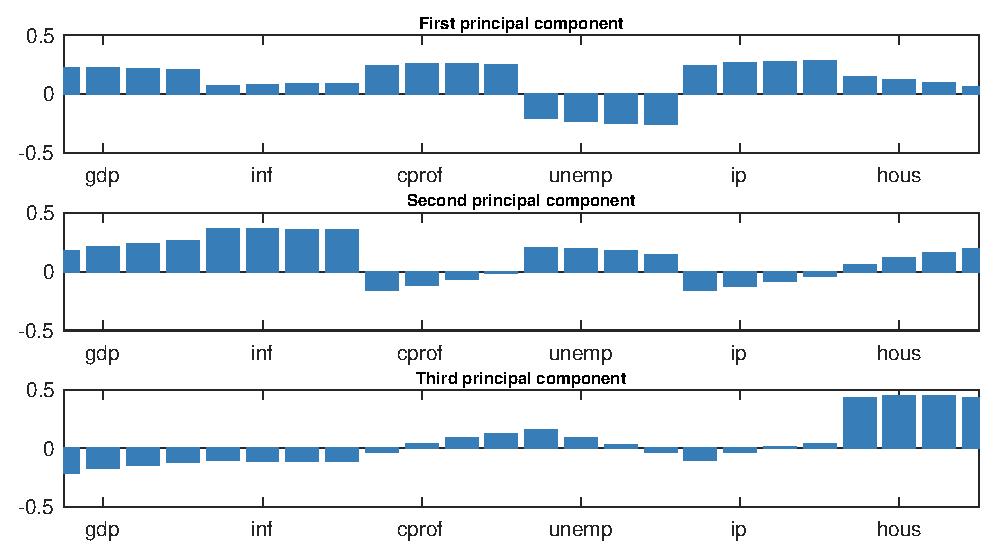
\includegraphics[scale=0.8]{Figures/e_pca_loadings.eps}
    \label{Fig:e_pca_loadings}
\end{figure}
The interpretation is naturally identical to the one obtained from the tabulated loadings, but the visualization may be more informative in some aspects. In particular, the graphical illustration naturally revels that loadings are similar in size for a particular fundamental across forecast horizons, albeit some heterogeneity in loading sizes are present. However, no loading is placed entirely on a particular forecast horizon for any of the macroeconomic fundamentals. 

%----------------------------------------------------------------------------------------------------------------------
% PLOTTING PCA LOADINGS
%----------------------------------------------------------------------------------------------------------------------

\clearpage
\section{Participation of individual forecasters}\label{sec:e_participation_of_individual_forecasters}
As mentioned in Section \ref{Sec:e_measuring_ebc}, the average number of participating forecasters in our sample is about $36$ per quarter. However, this number fluctuates over time as individual forecasters exit and enter the sample at various points in time.\footnote{See \cite{CapistranTimmermann2009} for a discussion on how best to deal with these exits and entries from a forecasting perspective.} To illustrate the participation, we consider in Figure \ref{Fig:e_participating_forecasters} the one-quarter ahead forecasts provided for the GDP variable over our sample period. 
\begin{figure}[htbp]
    \caption{
        \textbf{Participation of individual forecasters.} \newline
        This figure illustrates the participation of individual forecasters over our sample period. The blue dots represents a submitted forecasts from forecaster $i$ at time $t$. Forecaster IDs with no forecast submissions have been removed for easier readability of the figure. As a result, our notation of Forecaster ID need not correspond to the ID from the Survey of Professional Forecasters (SPF). The sample period starts in 1968:Q4 and ends in 2014:Q4.
    }
    \centering
    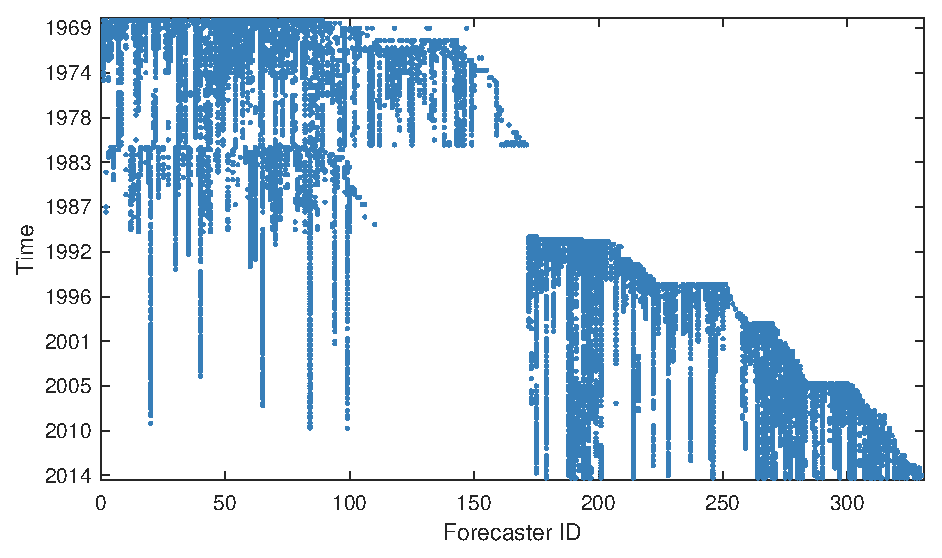
\includegraphics[scale=0.8]{Figures/e_participating_forecasters.eps}
    \label{Fig:e_participating_forecasters}
\end{figure}
Each dot represents a response by forecaster $i$, who are represented by a unique, but anonymous, forecaster ID, at time $t$. We see that the composition of the panel of professional forecasters vary over time and that individual forecasters frequently enter, exit, and re-enter the sample at various points in time. 

\end{appendices}
\end{document}

%----------------------------------------------------------------------------------------------------------------------
% END OF DOCUMENT
%----------------------------------------------------------------------------------------------------------------------